% =====================================================================
\subsection{Fase 6: niveles, cinemáticas y menús}

\subsubsection{Constructor de niveles a partir de mapas de texto}

Cada nivel se dibuja como un mapa de texto en el que cada carácter es una celda de 3 × 3~m
(Tabla~\ref{tab:caracteres}). Una segunda capa de letras agrupa las celdas en salas, y para cada sala
se definen su nombre, su color de luz, la esquina de su cámara principal y su tema de decoración. La
herramienta \cod{ConstructorNiveles} (menú \ruta{Nexus} \textrightarrow{} \ruta{Niveles}) convierte
esa descripción en el nivel 3D completo:

\begin{enumerate}
  \item coloca el suelo, las paredes donde el suelo toca un muro, las filas de racks, las puertas
        y los objetos;
  \item reparte las luces de cada sala por el método del punto más lejano, una cada cinco celdas
        aproximadamente;
  \item decora las salas según su tema;
  \item crea las cámaras fijas, sus zonas de cambio y los planos de interés, y verifica que todo el
        suelo quede cubierto;
  \item calcula la imagen del mapa para el inventario;
  \item coloca al jugador, los androides con sus rutas, los cadáveres con sus notas, las
        estaciones de carga y las cinemáticas.
\end{enumerate}

Así, los mapas sirven a la vez como diseño y como documentación de cada nivel, y un cambio en el
mapa se aplica reconstruyendo el nivel.

\begin{TablaAPA}{tab:caracteres}{Caracteres de los mapas de texto}
\begin{tabularx}{\linewidth}{P{1.4cm}LP{1.4cm}L}
\toprule
Carácter & Significado & Carácter & Significado \\
\midrule
\cod{\#} & Muro & \cod{.} & Suelo \\
\cod{=} \cod{|} & Fila de racks & \cod{S} & Inicio del jugador \\
\cod{T} & Terminal con mensajes & \cod{G} & Terminal de respaldo (guardado) \\
\cod{P} & Panel de fusibles & \cod{n} & Nota \\
\cod{R} \cod{B} & Puerta roja / azul & \cod{X} & Puerta sin energía \\
\cod{L} & Puerta libre & \cod{I} & Puerta de servicio (entrada) \\
\cod{E} & Ascensor o salida & \cod{D} & Disco Duro Maestro \\
\cod{k} \cod{a} & Tarjeta roja / azul & \cod{f} \cod{u} & Fusible / memoria USB \\
\cod{m} \cod{c} \cod{g} & Bebida, barrita, refrigerante & \cod{K} & Cadáver \\
\cod{Q} & Estación de carga & \cod{V} \cod{Y} & Máquinas expendedoras \\
\cod{M} \cod{W} \cod{b} & Mesa, escritorios, cajas & \cod{O} \cod{J} & Válvula / cápsula del jefe \\
\bottomrule
\end{tabularx}
\end{TablaAPA}

\subsubsection{Nivel 1: Cuarto de Mantenimiento}

El primer nivel es el tutorial (Figura~\ref{fig:mapa1}). El técnico entra por la puerta de servicio,
que se sella detrás de él, y debe seguir una cadena de objetivos que enseña las mecánicas del juego:

\begin{enumerate}
  \item La terminal de la sala de mantenimiento da la alerta y la misión.
  \item La oficina de seguridad no tiene energía: el panel del cuarto eléctrico necesita un
        fusible, que está en el almacén (Figura~\ref{fig:panel}).
  \item Con el fusible instalado se encienden las luces de la oficina y se abre su puerta; ahí está
        la tarjeta roja.
  \item La tarjeta abre la puerta roja de la sala de servidores, donde está el Disco Maestro~1
        (Figura~\ref{fig:puertaroja}).
  \item Al tomarlo suena la alarma y cuatro androides salen de sus estaciones de carga. El técnico
        solo tiene la bayoneta del cuerpo de Ramírez, así que la única opción es huir hasta el
        ascensor, al otro lado del nivel, en la cafetería.
\end{enumerate}

El nivel tiene 7:00 de refrigeración, una patrulla lenta y predecible que enseña a esconderse tras
los racks, y salas opcionales como la cafetería, con sus máquinas expendedoras, y el cuarto
eléctrico, con la primera terminal de respaldo (Figura~\ref{fig:salas1}).

\begin{figure}[!htbp]
  \caption{Mapa de texto del Nivel 1 y su plano generado para el inventario}\label{fig:mapa1}
  \centering
  \begin{minipage}{0.48\linewidth}\centering\footnotesize\linespread{1}\selectfont
\begin{verbatim}
###############
###############
#n.k#|...|#####
#.W.#|.D.|#####
#...#|K..|#####
##X####R#######
#Q.........Q###
##L##...##L####
#f..#.|.#u.P###
#mg.#...#.GQ###
#####.|.#######
#####...###V.Y#
###.T...n.#.ME#
##I.b.S...L..n#
###Qm...b.#KM.#
###############
\end{verbatim}
  \end{minipage}\hfill
  \begin{minipage}{0.48\linewidth}\centering
    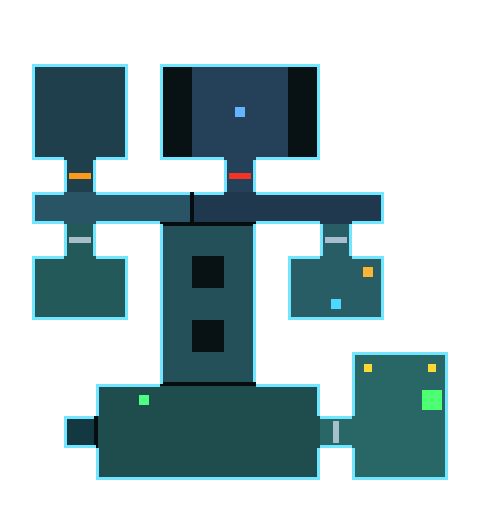
\includegraphics[width=\linewidth]{mapa_01_Mantenimiento.png}
  \end{minipage}
\end{figure}

\FiguraDoble{031_puerta-sin-energia-aviso.jpg}{032_panel-fusibles-reparado.jpg}{fig:panel}{Aviso de la puerta sin energía (izquierda) y panel de fusibles reparado (derecha)}{}

\Figura[0.75\linewidth]{034_puerta-roja-acceso-concedido.jpg}{fig:puertaroja}{La tarjeta roja abre la sala de servidores}{}

\FiguraDoble{063_mantenimiento-decorado.jpg}{064_oficina-seguridad-decorada.jpg}{fig:salas1}{Sala de mantenimiento (izquierda) y oficina de seguridad (derecha) decoradas}{}

\subsubsection{Nivel 2: Pasillos de Almacenamiento}

El segundo nivel fue diseñado y construido por Deisy Lorena Jiménez Martínez con la misma
herramienta de mapas de texto, a partir de un constructor propio del nivel
(Figura~\ref{fig:companera}). Es un laberinto de 21 × 18 celdas (63 × 54~m) formado por tres
franjas de racks en serpentina que se conectan por lados alternos, de modo que hay que recorrerlas
enteras, con salas arriba y abajo (Figura~\ref{fig:mapa2}). La iluminación de los pasillos es de
emergencia, verde y ámbar, con luces que titilan. El nivel empieza con 8:00 de refrigeración y el
núcleo al 86\,\%.

\Figura[0.9\linewidth]{companera_constructor_nivel2.jpg}{fig:companera}{Constructor del Nivel 2 en el editor de Unity}{Captura tomada por D. L. Jiménez Martínez durante la construcción del nivel.}

\begin{enumerate}
  \item La terminal de la sala de inicio da la misión.
  \item La tarjeta roja está en el almacén de carga, al este; abre la oficina de control, donde está
        la tarjeta azul.
  \item La tarjeta azul abre el núcleo de datos, que guarda el Disco Maestro~2.
  \item Con el disco suena la alarma y hay que volver por el laberinto hasta el ascensor, junto al
        inicio.
\end{enumerate}

La sala de respaldo es opcional y tiene la terminal de guardado, una memoria USB y objetos de
curación; la cafetería tiene las máquinas expendedoras. En este nivel aparecen los cuerpos de la
unidad táctica, que dan la pistola, la escopeta y la munición (Figura~\ref{fig:nivel2}). Hay siete
androides entre patrullas y estaciones de carga, con 84 puntos de vida en total, y la munición del
nivel suma unos 97 puntos de daño (26 balas y 5 cartuchos): alcanza para neutralizarlos a todos si
no se desperdicia, pero cada disparo fallado se nota, y lo que sobre pasa al Nivel 3.

\begin{figure}[!htbp]
  \caption{Plano del Nivel 2 generado para el inventario}\label{fig:mapa2}
  \centering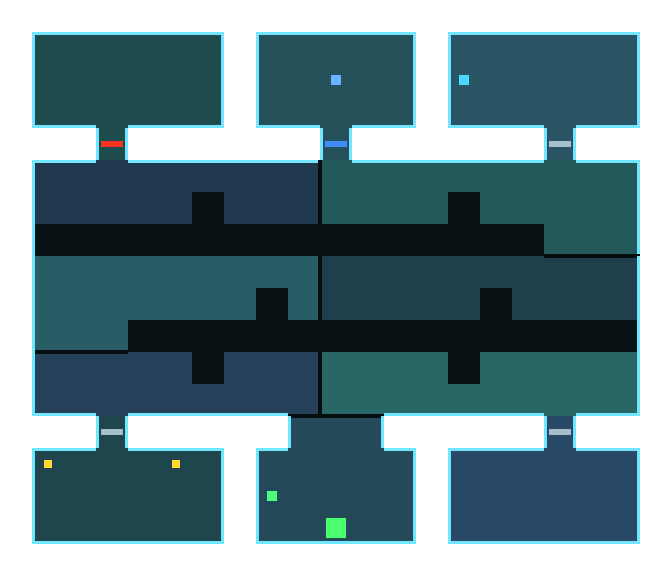
\includegraphics[width=0.6\linewidth]{mapa_02_Almacenamiento.png}
\end{figure}

\FiguraDoble{086_nivel2-sargento-escopeta.jpg}{098_nivel2-estacion-de-carga.jpg}{fig:nivel2}{Nivel 2: el sargento Ortiz con su escopeta (izquierda) y una estación de carga (derecha)}{}

\subsubsection{Nivel 3: Núcleo de Datos}

El último nivel es una sala central enorme y simétrica, con el núcleo en el centro rodeado por un
anillo de racks, tres alas (norte, oeste y este) y la sala de llegada al sur
(Figura~\ref{fig:mapa3}). El temporizador empieza en estado crítico, con 3:00 y el núcleo al
93\,\%. Cuatro androides patrullan en anillos alrededor del núcleo.

\begin{figure}[!htbp]
  \caption{Plano del Nivel 3 generado para el inventario}\label{fig:mapa3}
  \centering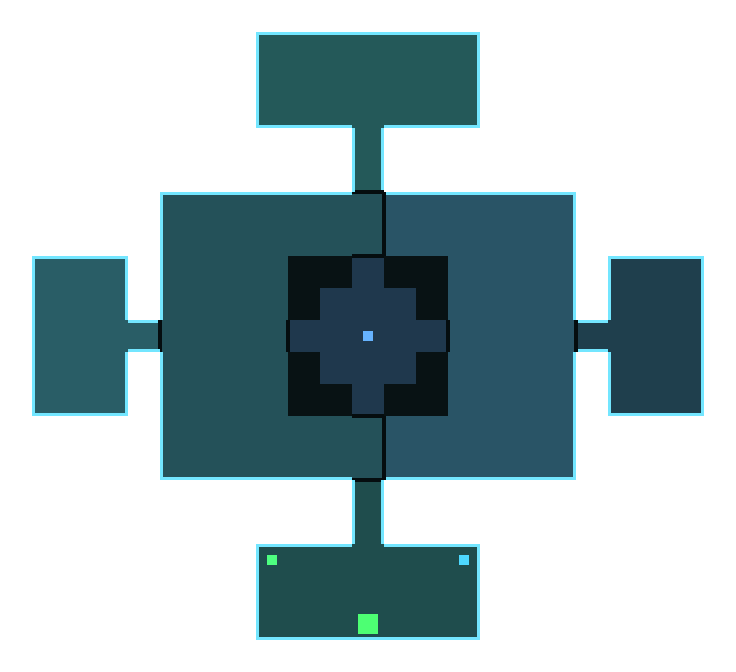
\includegraphics[width=0.6\linewidth]{mapa_03_Nucleo.png}
\end{figure}

El Disco Maestro~3 está protegido por un escudo térmico de tres anillos de energía, que se apaga
con un puzzle: abrir las tres válvulas de refrigeración, una en cada ala, en orden de menor a mayor
presión, como indica el manual de procedimiento de la sala de llegada (Figura~\ref{fig:valvula}).

\begin{itemize}
  \item Cada válvula tiene un manómetro que se lee al acercarse, y las presiones cambian en cada
        partida, por lo que hay que recorrer las alas y comparar.
  \item Si se abre una válvula en orden, la rueda gira, se apaga un tercio del escudo y el núcleo
        gana 60~s, una sola vez por válvula.
  \item Si se abre fuera de orden, se produce una sobrepresión: sale un chorro de vapor, todas las
        válvulas se cierran, el núcleo pierde 15~s y el estruendo atrae a los androides.
  \item Las notas de los cuerpos del nivel dan pistas sobre el orden.
\end{itemize}

\FiguraDoble{099_nivel3-valvula-manometro.jpg}{100_nivel3-alarma-disco.jpg}{fig:valvula}{Válvula del ala este con su manómetro (izquierda) y extracción del Disco Maestro~3 (derecha)}{}

Al tomar el disco se activa el jefe final, descrito en la fase~4. Con el jefe destruido, la salida
de emergencia permite iniciar el reinicio manual, que da paso a la cinemática final y a la pantalla
de Victoria.

\subsubsection{Cinemáticas}

El sistema de cinemáticas (\cod{Cinematica}) se hizo con el propio motor del juego: toma la cámara
y el personaje, muestra barras negras y subtítulos, oculta el HUD y detiene el temporizador y a los
androides. Cada plano define dónde empieza y termina la cámara, que se mueve con suavidad, qué
subtítulo aparece y qué ocurre en escena (caminar, mirar alrededor, abrir o cerrar una puerta,
encender la alarma, despertar a un androide). Los subtítulos usan el nombre del técnico elegido, y
cualquier cinemática se puede saltar. El constructor de niveles arma las cinemáticas a partir del
mapa.

\begin{itemize}
  \item \textbf{Entrada:} el técnico entra por la puerta de servicio, se pregunta \textquote{¿Qué
        pasó aquí\ldots?} mientras mira a su alrededor (con cinemática inversa de cabeza y torso) y
        la puerta se sella detrás de él (Figura~\ref{fig:intro}).
  \item \textbf{Alarma:} al extraer un disco, las luces pasan a rojo y laten, y la cámara muestra a
        las unidades encendiéndose una por una (Figura~\ref{fig:alarma}).
  \item \textbf{Final:} el sistema detecta los tres discos, las luces de alarma se apagan, las
        unidades caen desconectadas y se publican los registros del día 14
        (Figura~\ref{fig:final}).
\end{itemize}

\FiguraDoble{092_intro-puerta-servicio.jpg}{093_intro-que-paso-aqui.jpg}{fig:intro}{Cinemática de entrada: el técnico cruza la puerta de servicio (izquierda) y se pregunta qué pasó (derecha)}{}

\FiguraDoble{095_intro-puerta-sellada.jpg}{096_alarma-luces-rojas.jpg}{fig:alarma}{La puerta de servicio queda sellada (izquierda) y la alarma tiñe de rojo el nivel (derecha)}{}

\FiguraDoble{106_final-reinicio-manual.jpg}{107_final-se-acabo.jpg}{fig:final}{Cinemática final: el reinicio manual (izquierda) y el cierre de la historia (derecha)}{}

\subsubsection{Transición entre niveles}

El paso de un nivel al siguiente es una secuencia animada en el ascensor (Figura~\ref{fig:ascensor}).
Primero, las puertas se recogen hacia los marcos, sale la luz de la cabina y el técnico camina
hacia ella. Luego, el viaje transcurre dentro de una cabina de montacargas construida con primitivas
y con los materiales del propio ascensor, con una cámara fija en una esquina del techo: la cabina
arranca con un tirón, el indicador del panel baja de piso, la luz falla en dos momentos y la luz de
cada piso barre la cabina de abajo hacia arriba, hasta que frena de golpe. Mientras tanto, el nivel
siguiente se carga detrás de una pantalla negra y aparece con el sonido de las puertas y un
fundido. El viaje se puede saltar.

\Figura[0.95\linewidth]{114_transicion-ascensor.jpg}{fig:ascensor}{Las cuatro partes de la transición en el ascensor}{}

\subsubsection{Menú principal}

La escena \cod{00\_Menu} contiene el primer Canvas del juego, sobre un pasillo 3D del centro de
datos con racks y LEDs, los dos técnicos sobre plataformas con anillos de luz y un androide al fondo.
La cámara se mueve sola entre el plano del título y el del selector, como una cámara de seguridad.
El menú tiene cuatro pantallas:

\begin{enumerate}
  \item \textbf{Título} (Figura~\ref{fig:titulo}): logotipo con efecto de falla de pantalla,
        opciones del menú, el logo de la Universidad Central y un aviso de alerta que parpadea. La
        opción \textit{Continuar} aparece cuando hay una partida guardada, y \textit{Salir} se oculta
        en la versión web.
  \item \textbf{Selector de personaje} (Figura~\ref{fig:selector}, izquierda): el técnico elegido recibe un foco
        de luz, su anillo se enciende en cian y gira despacio, y a la izquierda aparece su ficha con
        su habilidad.
  \item \textbf{Informe de la misión} (Figura~\ref{fig:selector}, derecha): explica el objetivo, las amenazas
        y los controles, junto al retrato del técnico, y \textit{Iniciar misión} carga el Nivel~1.
  \item \textbf{Créditos} (Figura~\ref{fig:creditos}): materia, universidad, docente, semestre,
        integrantes y autores de los recursos. Sus textos y logos están en un archivo de datos que
        se edita desde Unity sin tocar el código.
\end{enumerate}

\Figura[0.85\linewidth]{118_titulo-logo-universidad.jpg}{fig:titulo}{Pantalla de título}{}

\FiguraDoble{051_selector-neyder.jpg}{053_briefing-mision.jpg}{fig:selector}{Selector de personaje (izquierda) e informe de la misión (derecha)}{}

\Figura[0.85\linewidth]{119_creditos-completos.jpg}{fig:creditos}{Pantalla de créditos}{}

El personaje elegido pasa al nivel mediante \cod{EstadoPartida}: un componente del jugador coloca
el avatar correspondiente antes que el resto de scripts, y como los dos avatares son Humanoid y
comparten el controlador de animación, el movimiento, las animaciones y la inteligencia artificial
funcionan igual con cualquiera.

\subsubsection{Pantallas de Game Over y Victoria}

El tercer Canvas es la pantalla final, presentada como una falla crítica del sistema Nexus y
animada paso a paso: destello y estática, tres anillos de radar que giran alrededor de un núcleo
que late, un título que se escribe con aberración cromática, el retrato del técnico con la leyenda
\textquote{Señal biométrica perdida}, un registro de terminal que cambia según la causa, un monitor
de pulso que se apaga, un informe del incidente y los comandos para reintentar, cargar la partida o
volver al menú (Figura~\ref{fig:gameover}). La Victoria usa la misma pantalla en verde y cian, con el
pulso estable (Figura~\ref{fig:victoria}). Todos sus gráficos se generan por código.

\FiguraDoble{047_game-over-anomalia-purgada.jpg}{048_game-over-colapso-termico.jpg}{fig:gameover}{Game Over por un androide (izquierda) y por colapso térmico (derecha)}{}

\Figura[0.8\linewidth]{049_victoria-sistema-restaurado.jpg}{fig:victoria}{Pantalla de Victoria}{}

% =====================================================================
\subsection{Fase 7: exportación}

Las tres versiones se compilaron desde el mismo proyecto con los perfiles de la fase~0. Windows usa
el entorno Mono; Android y Web usan IL2CPP, que convierte el código C\# a C++ antes de compilarlo
para procesadores ARM64 o para WebAssembly. Cada versión se probó al terminar: el ejecutable de
Windows se abrió y su registro no mostró errores (Figura~\ref{fig:windows}), y la versión web se
abrió en el navegador a través de un servidor local, porque un juego WebGL no se puede abrir con
doble clic, y se recorrió desde el menú hasta el Nivel~1 sin errores en la consola
(Figura~\ref{fig:web}). La plantilla web incluye el botón de pantalla completa que se necesita para
incrustar el juego en el artículo. La Tabla~\ref{tab:builds} resume las versiones finales.

\begin{TablaAPA}{tab:builds}{Versiones finales del juego}
\begin{tabularx}{\linewidth}{P{2.6cm}LP{2cm}P{2.4cm}}
\toprule
Plataforma & Archivo de entrega & Tamaño & Compilación \\
\midrule
Windows & \cod{Nexus\_Windows.zip} con \cod{Nexus.exe} & 97 MB & 0 errores \\
Android & \cod{Nexus.apk} (Android 8.0 o posterior, ARM64) & 75 MB & 0 errores \\
Web (WebGL) & \cod{Nexus\_Web.zip} para publicar en un servidor & 68 MB & 0 errores \\
\bottomrule
\end{tabularx}
\end{TablaAPA}

\Figura[0.8\linewidth]{windows_exe_menu.jpg}{fig:windows}{El juego ejecutándose en Windows}{}

\FiguraDoble{116_build-webgl-final-menu.jpg}{117_build-webgl-final-nivel1.jpg}{fig:web}{La versión web en el navegador: menú con el botón de pantalla completa (izquierda) y Nivel~1 (derecha)}{}
